\documentclass[review]{elsarticle}

\usepackage{bm, amssymb, amsmath, graphicx, mathtools, float}
\usepackage{lineno,hyperref,epstopdf,color}
\usepackage{tikz}
\usetikzlibrary{shapes,arrows}

\newcommand{\T}{^{\mbox{\tiny T}}}
\newcommand{\B}[1]{{\bm #1}}
\newcommand{\ds}{\displaystyle}
\newcommand{\kv}{$k$-vector}
\newcommand{\ndkv}{$n$-dimensional $k$-vector}
\newcommand{\Ndkv}{$N$-dimensional $k$-vector}
\newcommand{\NDKV}{$N$-Dimensional $K$-Vector}

\modulolinenumbers[5]

\journal{Journal of Applied Mathematics and Computation}

\bibliographystyle{elsarticle-num}

\begin{document}

\begin{frontmatter}

\title{Range searching in multidimensional databases using navigation metadata}


\author{David Arnas\corref{mycorrespondingauthor}}
\address{Massachusetts Institute of Technology, Cambridge, MA, 02139, USA.}\cortext[mycorrespondingauthor]{Corresponding author}\ead{arnas@mit.edu}
\author{Marcos Rodr\'{\i}guez}\address{Universidad de Zaragoza, Pedro Cerbuna 12, 50009 Zaragoza, Spain.}


\begin{abstract}
This work presents a new range searching algorithm for multidimensional databases. The proposed methodology is based on the idea of generating a navigation metadata structure, complementary to the database, that eases the navigation between the elements of the database. This metadata structure  can be adapted to different problems and it is generated in a one time pre-procesing effort for each database. This work contains a complete description of the algorithm, including a study of its searching performance under different conditions compared with a brute force approach.
\end{abstract}

\begin{keyword}
Computer Science \sep Range Searching Techniques \sep Multidimensional Spaces \sep Data Structures
\end{keyword}

\end{frontmatter}

\linenumbers

\section{Introduction}
\label{sec:intro}

Many problems in science require the study of vast amounts of data, being this an increasing necessity with the evolution of technology available. Examples of that include the study of data from scientific experiments, the identification of iso-surfaces in physics problems, the fast access to information from databases, or the classification of population in a statistical study.

This work focuses on the problem of performing orthogonal range searching in multidimensional static databases. In particular, the problem that this manuscript deals with is the following: having a multidimensional database of $n$ elements, the objective is to find all of those elements that are contained in a given searching range $[a_i,b_i]$, where $a_i$ and $b_i$ are respectively the lower and upper bounds of the searching range in each dimension. In general, this kind of search can be performed by a brute force approach consisting on checking, one by one, all the elements of the database to determine if they are included in the searching range. By doing this, the searching time required by the algorithm is directly proportional to $n$, the number of elements in the database. This implies that the larger the database, the slower this kind of algorithms perform their search. As a result, a wide variety of methodologies have been proposed to improve this limiting behavior. Examples of these algorithms are the projection method~\cite{basic} which consists on performing the search in a database sorted in one dimension of the problem , the grid files method~\cite{grid} which is based on defining a grid to ease the searching process, or the many algorithms based on tree data structures~\cite{making,barnes,olson} such as the $b$-tree~\cite{btree}, the quad tree~\cite{quadtree}, the $k$-d tree~\cite{Bentley}, the $R$-tree~\cite{rtrees}, or the $Kdb$-tree~\cite{kdbtree}. However, there is a wider variety of methodologies~\cite{willard,lueker,alstrup,arya,ndkv} based on different approaches to the problem~\cite{agarwal,Chazelle}.

This manuscript introduces the cell web algorithm, a new technique devised for the fast retrieval of all the elements in a multidimensional static databases contained in an orthogonal searching range. This algorithm is lies on the idea of defining a grid in a set of dimensions of the database and provide some navigation metadata between the different cells of the grid. In order to ease the navigation between cells, a representative element in each occupied cell of the grid is selected. These representative elements are used to identify the positions in memory of the elements inside the cells previously defined. That way, the algorithm is able to move through the different regions of the searching space in a fast and easy process. In addition, if the number of cells defined by the algorithm is too big (due to a high number of dimensions) when related to the number of elements of the database, the algorithm performs the search in a projected space defined in a subset of dimensions of the problem.

The cell web algorithm performs the retrieval of elements based on the grid defined during the pre-processing effort. This means that unless applied to problems where an approximated search is requested, a post-processing performed in the elements retrieved is required. This post-processing follows a brute force scheme, where the algorithm first assesses the possible dimensions not covered by the defined grid, and then it continues by checking the remaining dimensions. This allows the algorithm to match the searching range while significantly reducing the number of elements to study during the post-processing.

This work is organized as follows. First, this manuscript presents a general overview of the algorithm containing the conceptual idea behind it. Second, a more detailed description of the methodology is shown. This exposition includes the study of the database structure, the generation of the navigation metadata, and the searching process of the algorithm. Finally, the complexity and speed performance of this technique is studied. In that regard, the speed performance is compared with a brute force approach in order to have a clear comparison reference for the methodology.


\section{Cell Web Algorithm}
\label{sec:algorithm}

\subsection{General overview}
\label{sec:idea}

The algorithm proposed in this manuscript lies on the idea of generating a data structure containing a set of navigation directions between the elements of the database that will be used to retrieve in a simple and fast methodology all the elements contained in a given range. The algorithm requires to perform a one time pre-processing effort consisting on sorting the database, following a given criterion, and then generating the associated metadata which will allow the direct navigation between elements of the database. However, due to the fact that the number of metadata required would increase exponentially with the number of dimensions of the database, this navigation data is generated for a subset of these dimensions. That way, the pre-processing effort is performed only once for each database, being the results of it stored. The basis of the pre-processing can be summarized in the following steps:
\begin{itemize}
  \item Select a subset of dimensions in which a grid is defined.
  \item Define a sorting criterion for the elements of the grid.
  \item Sort the database according to the criterion selected.
  \item Attach complementary metadata for the fast navigation between the elements in the database, taking into account that this metadata could be only defined in a subset of dimensions from the original database.
\end{itemize}

Once the pre-processing is done, it is then possible to perform the orthogonal search. In order to do that, the algorithm first transforms the orthogonal search into a search based on the previously defined grid. Note that since, in general, the searching range does not need to match with the defined grid, the algorithm has to impose that the original searching interval is strictly contained inside the this equivalent search. This means that the algorithm is able to assure that the process will retrieve at least all the elements inside the searching interval. That way, the algorithm can focus on the identification of the cells that define the searching range instead of in the searching range itself. For simplicity, we will refer to these cells as range cells.

After this range transformation, a binary search technique is used to find an element from the first range cell defined by the searching range. Then, from the position of this first element, the navigation metadata is used to identify the elements that are adjacent in memory and contained in the range cells. However, not all the elements in the searching range will be in general adjacent in memory. Therefore, in order to identify these non-adjacent elements, the algorithm makes use of the navigation metadata to search the first element contained in the next occupied range cell not adjacent in memory. Once this element is identified, the algorithm retrieves again all the elements that are adjacent in memory and contained in the range cells repeating the process.

This searching process continues until all the range cells are evaluated. At this moment, not all the elements retrieved are part of the searching range. This is due to two reasons. First, it is not possible to obtain a perfect match between the original searching range and the grid generated. Second, and if dealing with databases with a many dimensions, the navigation metadata is only defined in a subset of these dimensions. Therefore, a post-processing effort is performed to identify which of the elements retrieved are outside the searching range. Note that following this process, the majority of the database will be, in general, discarded in the initial phase of the search.

In order to make the methodology clearer, a summary of the steps followed by the searching process is included in the following lines:
\begin{itemize}
  \item Transformation of the searching range into a search based on cells that are the best approximation of the searching range and fully contain it. These cells are defined by the grid generated during the pre-processing. Figure~\ref{Fig:basis} shows a random three-dimensional database that has been distributed in a $3\times3\times3$ grid. This means that each of the three grids presented in the figure correspond to the three different layers in which the third dimension is distributed. Moreover, Figure~\ref{Fig:basis} shows the range cells, which are represented by the gray areas in the database.
  \item Searching of the first element in the range using a binary search technique applied to the grid generated during the pre-processing. This first element is represented in Figure~\ref{Fig:basis} with a star.
  \item Retrieval of the elements inside the range cells and that are adjacent in memory to this first element. The navigation between elements located in adjacent memory is performed using the navigation metadata and is represented in Figure~\ref{Fig:basis} by dashed lines.
  \item The navigation metadata is used to identify the location of the first element of the next searching cell to study. In Figure~\ref{Fig:basis} this navigation is represented by solid lines.
  \item Retrieval of all the elements of the database that are adjacent in memory and contained in the range cells. Afterwards, the navigation process is repeated until all elements inside the range cells are retrieved.
  \item A post-processing effort is performed in order to assure that all the elements retrieved are contained in the original searching range.
\end{itemize}

\begin{figure}[!h]
\begin{center}
	\begin{tikzpicture}[x=2.5cm,y=2.5cm]
	% \tikzset{pto/.style={circle, draw,inner sep = 0, outer sep = 0, minimum size=0.3mm}}
	\tikzset{pto/.style={circle, draw, fill, inner sep = 0, outer sep = 0, minimum size=0.6mm}}
	\foreach \k in {0,1} {
		\begin{scope}[shift={(1.2*\k, 0)}]
		\fill[gray!15!white] (0.3333,0) rectangle +(0.66666,0.66666);
		\end{scope}
	}
	\foreach \k in {0,1,2} {
		\begin{scope}[shift={(1.2*\k, 0)}]
		\input{points\k.tex}
		\foreach \j in {0,0.33333,0.6666666,1} {
			\draw[thin] (0,\j) -- +(1,0);
			\draw[thin] (\j,0) -- +(0,1);
		}
		\end{scope}
	}
	\draw[-to, dashed] (P3) edge (P8) (P8) edge (P7) (P7) edge (P9);
	\draw[-to, dashed] (P1) edge (P0) (P0) edge (P2);
	\draw[-to, dashed] (P23) edge (P24) (P24) edge (P25);
	\draw[-to, dashed] (P18) edge (P20) (P20) edge (P21);
	\draw[thick, gray!15!white,rounded corners = 5pt, -to] (P3) -- ++(-0.1,0) |- (P1);
	\draw[rounded corners = 5pt, -to] (P3) -- ++(-0.1,0) |- (P1);
	\draw[thick, gray!15!white,rounded corners = 5pt, -to] (P1) -- ++(0,-0.4) -| (P23);
	\draw[rounded corners = 5pt, -to] (P1) -- ++(0,-0.4) -| (P23);
	\draw[thick, gray!15!white,rounded corners = 5pt, -to] (P23) -- ++(-0.1,0) |- (P18);
	\draw[rounded corners = 5pt, -to] (P23) -- ++(-0.1,0) |- (P18);

	\node[draw,star,star points=5,star point ratio=1.8, minimum width = 3mm,inner sep = 0] at (P3) {};

	\begin{scope}[shift={(3.5,0.8)}]
	\node[right,draw,fill=gray!15!white,minimum width = 4mm] (D) {};
	\node[right] at (D.east) {\scriptsize Cell searching range};
	\node[right, draw,star,star points=5,star point ratio=1.8, minimum width = 3mm,inner sep = 0] at (0.015,-5mm) (A) {};
	\node[right] at (A.east)  {\scriptsize First Output Point};
	\node[right, minimum width=4mm] (B) at (0,-10mm) {};
	\draw[-to, dashed] (B.west) -- (B.east) node [right,inner sep = 0.5mm] {\scriptsize {Adjacent memory navigation}};
	\node[right, minimum width=4mm] (C) at (0,-15mm) {};
	\draw[-to] (C.west) -- (C.east) node [right,inner sep = 0.5mm] {\scriptsize {Non adjacent memory navigation}};

	\end{scope}


	\end{tikzpicture}
\end{center}
\caption{Schematic representation of the searching process.}\label{Fig:basis}
\end{figure}


\subsection{Data structure}
\label{sec:structure}

This subsection describes the data structure used and how the pre-processing effort of the algorithm is performed. As seen previously, the algorithm requires to generate a data structure during the pre-processing that allows a fast searching process. This data structure contains both the information of the elements that will be searched, and also some navigation metadata that allows a simple navigation through the database.

Without lost of generality, in this work a normalized space is considered, where all the coordinates of the database elements range in the interval $[0,\: 1]$. If spaces of other sizes are used, the methodology can be still applied by a normalization of the space or, alternatively, by an adjustment of the methodology to the size of the space considered.

Following the process presented in the previous subsection, the first step of the algorithm is to select a subset of dimensions where the grid is defined. In that regard, and should the algorithm not being focused on speed, the size of the grid could have been left free, extending it to all the dimensions presented in the space. However, the proposed algorithm aims to be fast, and so, we have to impose a boundary in the number of dimensions in which the grid is defined. That way, the number of resultant hyper-dimensional cells that the computer has to study is significantly reduced, making the algorithm faster as we will see in Section~\ref{sec:complexity}. Moreover, we are interested in defining grids whose cells have a mean number of elements bigger than one. There are two reasons for that. First, the algorithm is able to ignore the cells that are completely empty. Second, the navigation is performed between cells, which implies that the number of occupied cells determines the number of range cells that will be evaluated during the search.

Let $n$ be the amount of elements contained in a database of dimension $d$. Then, if a uniform distribution of elements is assumed where $n_c$ different cells in the length of each dimension are defined, the resultant number of cells that can be generated in the whole searching space is equal to $n_c^d$. As it can be seen, the number of cells increases exponentially with the number of dimensions of the problem, and thus, if the number of dimensions is big enough, the number of cells can be much larger than the size of the database. This causes the navigation through elements to become equivalent to the navigation through cells, and thus, equivalent to use a brute force methodology. For this reason, in order to improve the performance of the methodology for those cases, we select a subset of dimensions such that:
\begin{equation} \label{eq:subdim}
d_s \leq \left\lfloor\log_{n_c}n\right\rfloor,
\end{equation}
where $\lfloor x \rfloor$ is the round down value of $x$, and $d_s$ is the number of dimensions selected from the available dimensions $d$. Note that the definition of $d_s$ provided determines the boundary situation where each cell contains in average only an element from the database. For this reason, and for most applications, the number of selected dimensions should be lower than these boundary value. These dimensions can be chosen freely, and thus, if the problem is more sensitive to certain dimensions, those should be the dimension in which to define the grid.

As a result of the grid defined, it is possible to easily identify the cell in which each element of the database is located. Let $i$ be a given dimension from the subset $d_s$, and let $x_i$ be the normalized coordinate in that dimension of an element of the database. Then, the location of that element in the grid is obtained using the following expression:
\begin{equation}\label{eq:v_score}
s_i = \lfloor x_i n_c \rfloor, \quad \forall \: i\in\{1,\dots,d_s\},
\end{equation}
where $s_i$ represents the relative position of the cell in the grid using vector notation. This means that each hyper-dimensional cell of the grid is assigned with a different value of $\mathbf{s} = (s_1, s_2, \dots, s_i, \dots, s_{d_s})$, which for the purpose of this work, is called score. Note that although each cell has a different score, two different elements of the database can present the same score, that is, they are contained in the same cell.

While doing the search, the algorithm requires to perform a binary search and some navigation through the database. In order to do that, it is first required to have a database sorted in some way. Unfortunately, it is well known that, in general, and contrary to what happens in one dimensional spaces, there is not a clear order when dealing with multidimensional spaces. This means that a criterion has to be defined in order to sort the database. For the case of the proposed algorithm, an integer based score has been selected. The idea behind this methodology is to use the cell based score defined in Eq.~\eqref{eq:v_score} to sort the database. In particular, the integer score ($s_t$) of a cell element is defined as:
\begin{equation}
s_t = \sum_{i = 1}^{d_s}s_in_c^{i-1}.
\end{equation}
As it can be seen, components of the score with a larger $i$ index have more impact in this quantity. For this reason, the algorithm performs score comparisons by a series of comparisons between the components of the vector score with the same index, that is, $s_i$ with $i\in \{1,\dots,d_s\}$, starting with the component that presents the largest index. That way, once one of the scores presents a component bigger than the other, it is possible to derive that such score is bigger. Following this criterion, it is possible to sort the whole database using an algorithm such as mergesort or quicksort. Note that elements with the same score do not have any priority between them and as such are sorted according to the original database.

The next step in the pre-processing requires to define a representative for each cell containing at least an element from the database. This representative is chosen in such a way that it is the first element in memory that presents a given score. This definition has two purposes. First, it allows to identify unequivocally each cell of interest with just one element of the database. Second, it allows to identify the first location in memory where the elements have a given score. The information of the cell representatives for each element are stored as navigation metadata for the algorithm. Additionally, and in order to allow the fast navigation through elements that are adjacent in memory, the representatives of the previous and next occupied cells in memory are also stored as part of the navigation data. Note that in this way the algorithm can navigate without problems in the first dimension of the problem through all the database.

The final step in the pre-processing is to generate the navigation metadata that allows to relate elements that are not adjacent or close in memory, or in other words, this metadata aims to ease the navigation in the dimensions where $i\in\{2,\dots,d_s\}$. In that sense, it is worth noticing that during the searching process, the algorithm starts in the elements that have the lowest score in the searching range and continues with the retrieval of elements in ascending value of score. This means that we are only interested in the navigation information related to an increasing evolution of score. This means that, for each database element, we require to define $(d_s-1)$ navigation components that are related with each dimension not covered before. In particular, and for a given element, the navigation metadata for the dimension $i$ stores the amount of elements located in the hyper-cell of dimension $i-1$ and that contains that element. In other words, given a vector score $\mathbf{s}$ and a given dimension $i$, the algorithm counts the number of elements from the database with a vector score $\mathbf{s'}$ such that:
\begin{equation}\label{eq:navscore}
s'_k = s_k \quad \forall  k \in\{i,...,d_s\}.
\end{equation}
For instance, if the second dimension is considered, this metadata stores the information of how many elements are located inside the row of cells containing associated with that element. For the third dimension, instead of evaluating a row of cell, the algorithm has to evaluate the plane of cells containing the given element. It is important to note that this navigation is defined between cells, and thus, it is not required to compute this metadata for each individual element from the database. Moreover, since the amount of elements contained in a plane of cells is equivalent to the sum of the number of elements contained in all the cell rows of that plane, this pre-processing can be easily done by just counting once the number of elements per cell row and then extrapolating the result to other dimensions. For instance, in Fig~\ref{Fig:basis} the metadata stored for the reference element marked with a star will be the number of elements per line (7 elements), and the number of elements in the plane (18 elements).

Once the previous computations are finished, the pre-processing of the algorithm is completed for a given database. At this point, each element of the database has access the following information:
\begin{itemize}
	\item Coordinates of the element: an array of size the number of dimensions that contains the coordinates of the elements in the searching space.
	\item Cell score: an integer array of size the number of dimensions that identifies the grid cell in which the element is located.
	\item Cell representative: an integer number that provides the location in the database of the cell representative of the element.
	\item Previous cell representative: an integer number that provides the location of the cell representative of the previous cell adjacent in memory.
	\item Next cell representative: an integer number that provides the location of the cell representative of the next cell adjacent in memory.
	\item Cell navigation: an array of integer numbers sized the number of selected dimensions minus one $(d_s - 1)$ that contains the number of elements of the database satisfying Eq.~\eqref{eq:navscore}.
\end{itemize}


\subsection{Searching process}
\label{sec:search}

Having done the pre-processing effort, it is now possible to perform the searching using the proposed algorithm. The first step in the searching process is to transform the searching intervals into an equivalent search in cells. This is done using the grid score defined in Eq.~\eqref{eq:v_score}, taking into account that the algorithm has to assure that the search cells contain the whole searching range. This means that if the limit of the range lays inside a given cell, the algorithm will have to evaluate the whole cell to be sure that no correct element was removed. In addition, since we are dealing with orthogonal searching and the range has been transformed into a search in cells, it is possible to define the whole cell range by identifying the scores of the two opposite vertices. Let $[a_i, b_i] \quad \forall \: i\in\{1, \dots, d_s\}$ be the searching range in the dimensions selected during the pre-processing, where $\mathbf{a}$ contains the lower bounds while $\mathbf{b}$ the upper bounds of the ranges. Then, the range cells correspond to the subset whose score fulfills:
\begin{equation}
\lfloor a_in_c \rfloor \leq s_i \leq \lfloor b_in_c \rfloor\ \quad \forall \: i \in \{1,\dots,d_s\}.
%s_i \in \{\lfloor a_in_c \rfloor,\dots, \lfloor b_in_c \rfloor\} \quad \forall \: i \in \{1,\dots,d_s\}.
\end{equation}
This means that it is possible to identify the whole searching range with just the initial and final range cells of the searching range, that is, $s_i = \lfloor a_in_c \rfloor$ $\forall \: i \in \{1,\dots,d_s\}$, and $s_i = \lfloor b_in_c \rfloor$ $\forall \: i \in \{1,\dots,d_s\}$ respectively.

Once the range cells are identified, a binary search is performed in order to find an element in the database (and, subsequently the representative) that has the same score that the initial cell of the searching range, that is, $s_i = \lfloor a_in_c \rfloor$ $\forall \: i\in\{1,\dots,d_s\}$. If such score does not exist in the database, the algorithm retrieves the closest element with a score bigger than the one sought. From this first element, the algorithm now retrieves all the elements that are adjacent in memory and inside the range cells identified in the previous step. The process is done as follows: instead of checking if the adjacent elements lay inside the searching interval, the algorithm only assesses the adjacent cells using the metadata information. This means that the number of operations is reduced proportionally to the number of elements in each cell. Moreover, it is worth noticing that since the metadata allows to navigate between cells containing database elements, cells that are empty are completely ignored.

Then, the algorithm focuses on finding the next subset of adjacent elements. This is done by the use of a cell counter, and the navigation metadata. The cell counter works as a digital clock and its goal is to set the target cell. On the other hand, the navigation metadata allows to first obtain an element located close to the target cell, and then to identify the representative of the target cell in a linear search that in general takes a small number of steps. This means that the algorithm has a very good first approximation on where the representatives of the next range cells are located. Then, by using the information of the next and previous cell representative, it is very simple to identify the element sought. In other words, the navigation metadata helps to mimic the movements provided by the cell counter but in the database, since it contains the information of the basic movements that the clock can provide.

Once this first element of the subset is identified, the algorithm retrieves all the adjacent elements in memory that are inside the searching range, following the same process explained before. The process of searching for the next subset of adjacent elements in memory and then performing their retrieval is continued until all range cells are evaluated. This condition is equivalent to continue the process until the algorithm reaches the cell defined by the score $s_i = \lfloor b_in_c \rfloor$ $\forall \: i\in\{1,\dots,d_s\}$.

After this process is performed, there will be, in general, elements retrieved that are outside the searching interval. This is caused by two factors. First of all, not all dimensions have been assessed yet. Second, the boundaries defined by the range cells may not present a perfect match with the searching range. For those reasons, a post-processing effort is performed. This post-processing is based on a brute force approach where the algorithm first assess the boundaries in the remaining dimensions, and then, it checks the dimensions studied during the cell process.



\section{Algorithm complexity}
\label{sec:complexity}

One of the most interesting performance metrics for searching algorithms is the algorithm complexity, which is the focus of this section. To that end, a statistical approach is performed. Let $d$ be the number of dimensions of a database of size $n$, and let $d_s$ be the subset of dimensions where the grid of the algorithm is defined. In addition, let $n_c$ be the number of cells in each dimensional direction. This means that the total number of cells defined in the space is $n_c^{d_s}$. Therefore, there is on average $n/n_c^{d_s}$ elements per defined cell.

The objective now is to determine the number of cells that must be evaluated, since that will identify the average number of elements that will be required to check during the post-processing. In a uniform distribution, the ratio between the elements retrieved ($k$) and the size of the database is proportional, in average, to the ratio between the number of cells evaluated and the total number of cells or, in other words, to the fraction of the hyper-volume covered by the cells. This means that if all dimensions were studied, the following relation should be fulfilled:
\begin{equation}
\displaystyle\frac{k}{n}\approx\left(\frac{k_c}{n_c}\right)^d;
\end{equation}
where $k$ is the amount of elements to be retrieved, and $k_c$ the average number of cells inside the searching range for a given dimension. Therefore, it is possible to determine the average range in cells that will be studied:
\begin{equation}
k_c\approx n_c\left(\displaystyle\frac{k}{n}\right)^{(1/d)}.
\end{equation}
Thus, the number of cells to evaluate must be proportional to the space defined under this range in a $d_s$ space, that is:
\begin{equation}
\left[n_c\left(\displaystyle\frac{k}{n}\right)^{(1/d)}\right]^{d_s},
\end{equation}
and since we already know the average number of elements inside a given cell, the total number of elements that are required to be evaluated is:
\begin{equation}
\displaystyle\frac{n}{n_c^{d_s}}\left[n_c\left(\displaystyle\frac{k}{n}\right)^{(1/d)}\right]^{d_s},
\end{equation}
which provides an average complexity of:
\begin{equation}\label{eq:complexity}
\mathcal{O}\left(\displaystyle\frac{n}{n_c^{d_s}}\left[n_c\left(\displaystyle\frac{k}{n}\right)^{(1/d)}\right]^{d_s}\right) = \mathcal{O}\left(n\left(\displaystyle\frac{k}{n}\right)^{(d_s/d)}\right).
\end{equation}

Note that in order to start the retrieval of elements, the algorithm also requires to identify the first element from the searching range through a binary search technique. This search has a complexity of $\mathcal{O}\left(d_s\log{n_c}\right)$, which has a much smaller complexity than the one derived from the post-processing of the elements retrieved. Therefore, the overall average complexity of the algorithm is $\mathcal{O}(n\left(k/n\right)^{(d_s/d)})$.


\section{Speed performance}
\label{sec:performance}

In this section we present a study on the speed performance of the algorithm presented and compare it with a brute force approach. In that regard, two different databases containing 8 million elements are used. The first database is generated based on a uniform random distribution of points in the space. The second database is based on the colored image seen in Figure~\ref{fig:tulip}. There, each element corresponds to a pixel in the image, while the dimensions of the searching space correspond to the position of the pixel in the color space (red, blue and green). If a larger number of dimensions is required, these components are repeated as new dimensions.  That way, we present the speed performance of the algorithm both for uniform and non uniform databases.

\begin{figure}[h!]
	\centering
	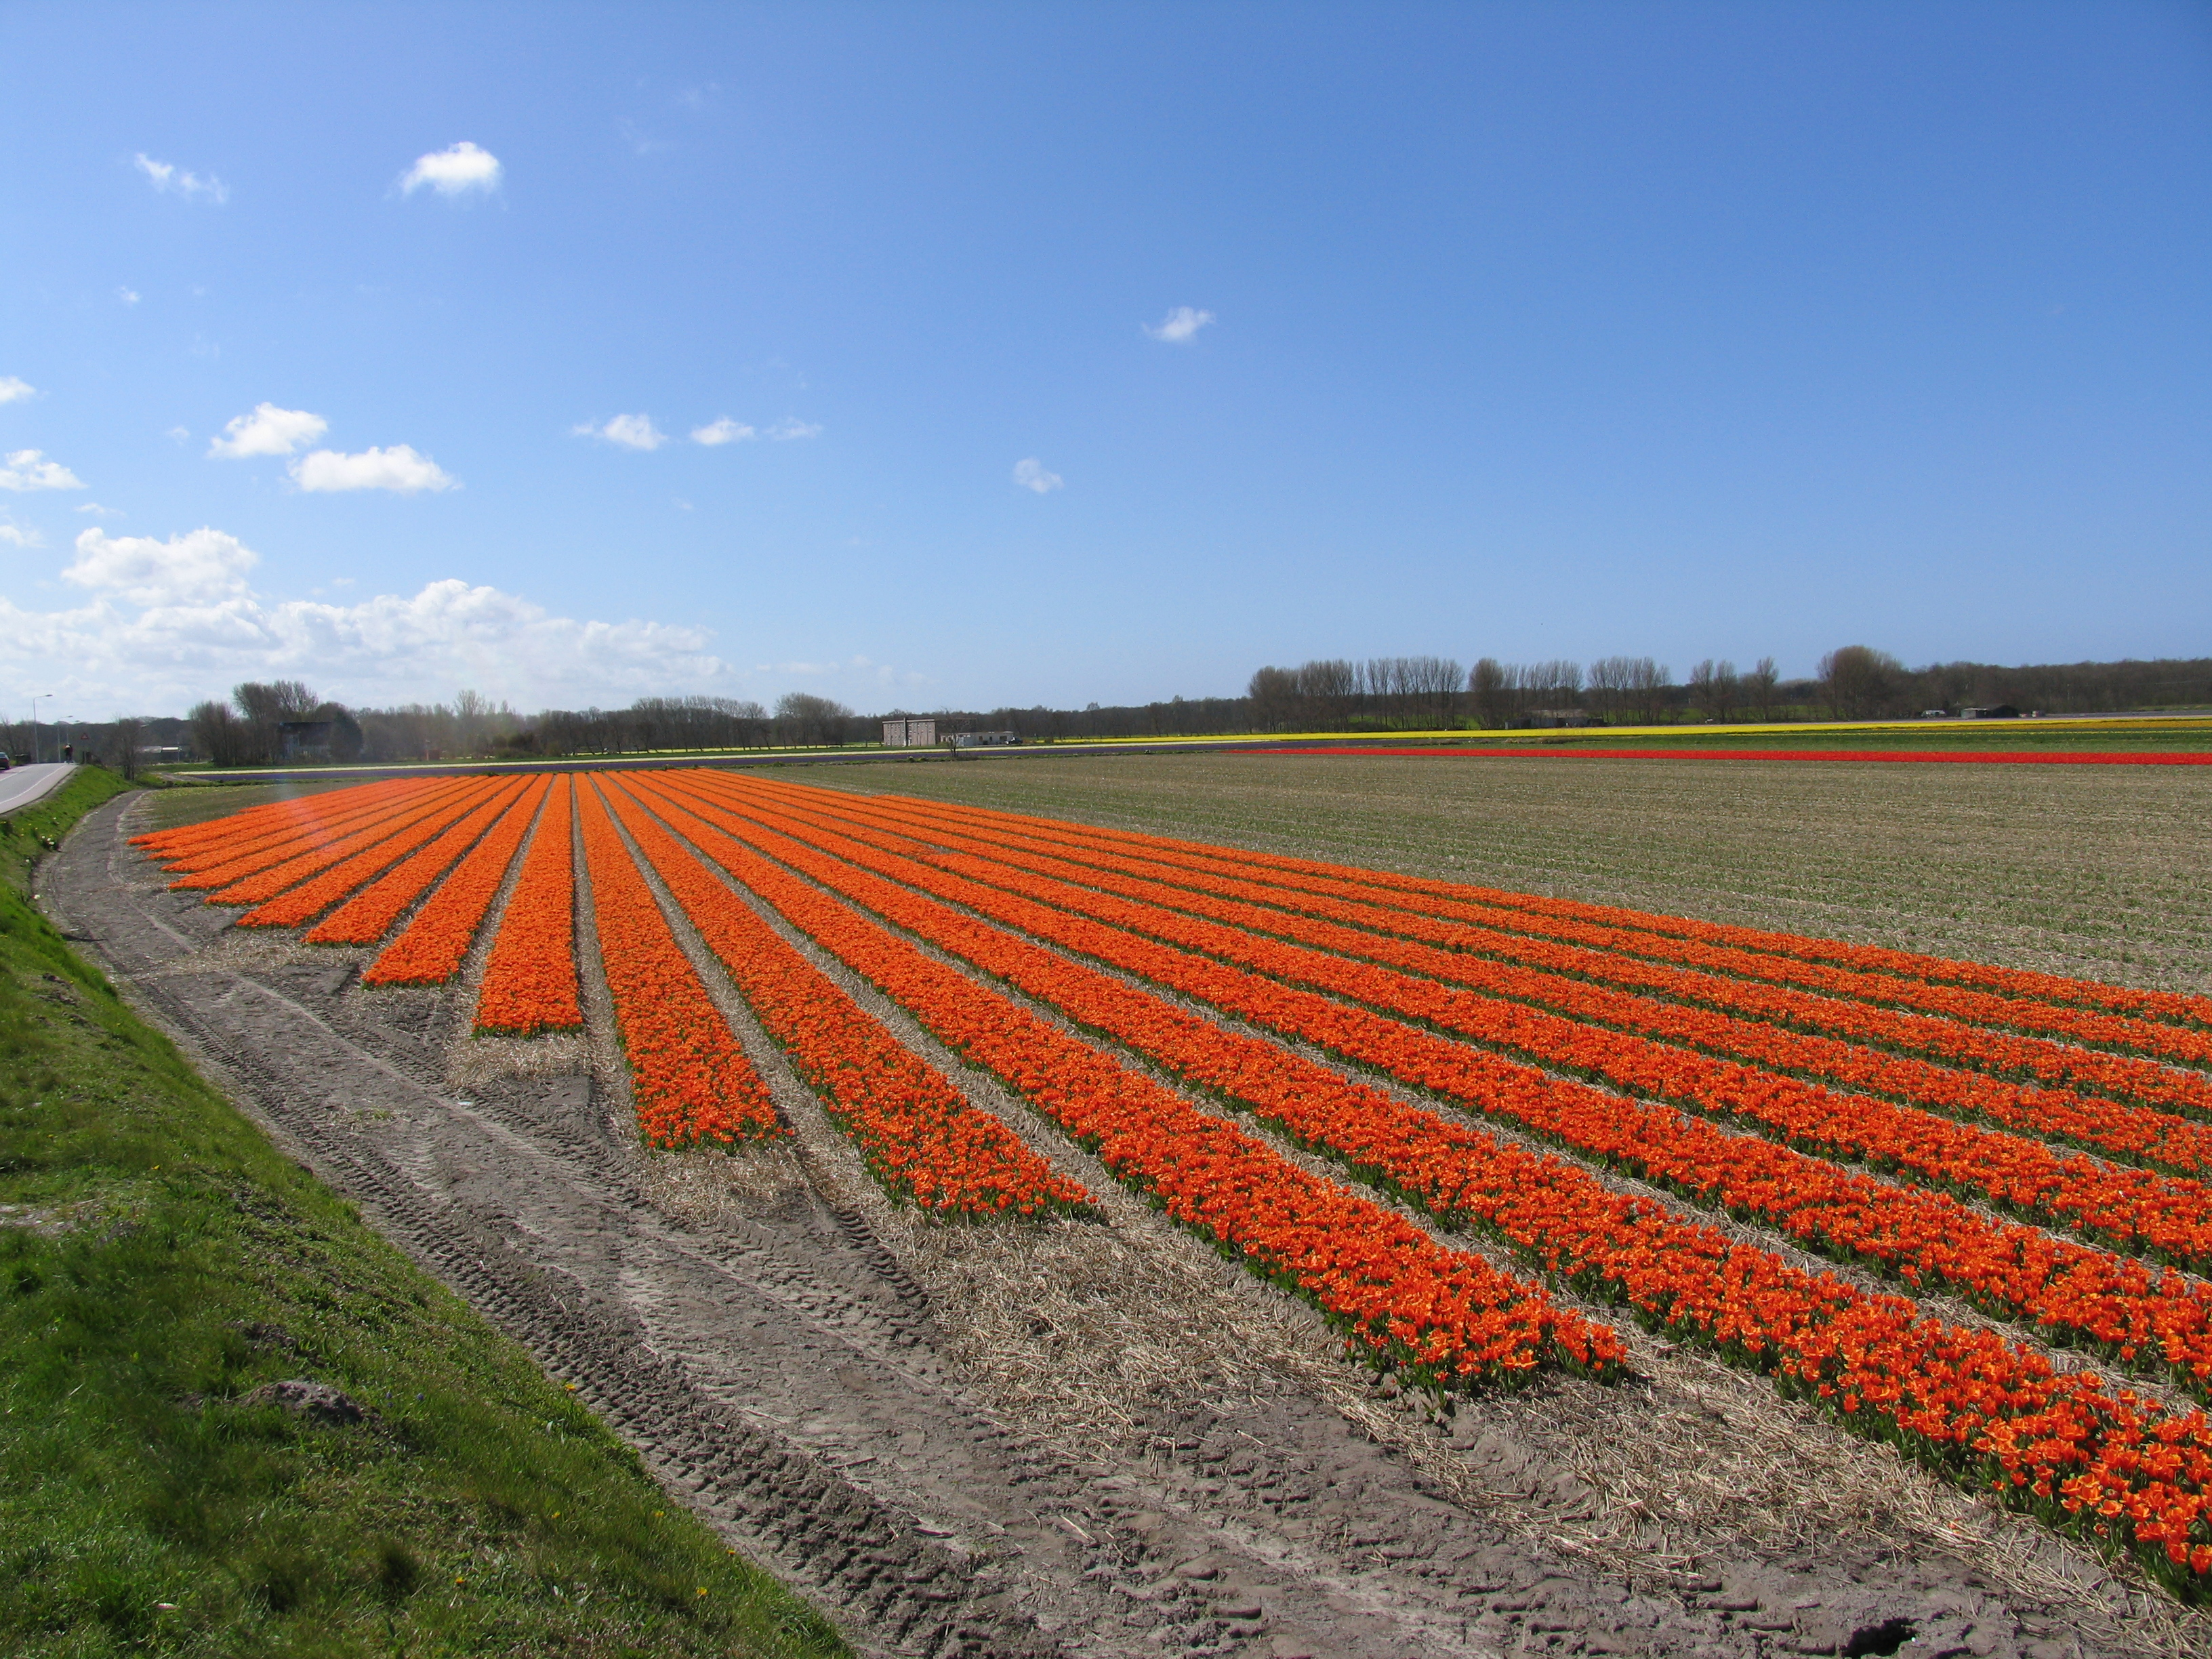
\includegraphics[width=0.95\textwidth]{t01.pdf}
	\caption{Image used for generation of the non-uniform database.}
	\label{fig:tulip}
\end{figure}

For this study, a single threaded implementation of the algorithm was used, being all the tests performed in the same computer under similar conditions. All the test were performed with $n_c = 100$ and included the post-processing to check all the elements retrieved. In the figures presented below, we compute the relative speed, that is, the ratio between the time that the algorithm takes to perform the search when compared to a brute force approach. That way, having a relative speed of 1 means that the algorithm is running at the same speed as the brute force approach, while if the relative speed is lower, the algorithm is faster. This means that the lower the value for this result, the faster the algorithm is.

Figure~\ref{fig:dimensions} shows the relative speed of the algorithm when compared with a brute force approach for different number of dimmensions of a given database. In this figure, the number of elements retrieved in each search is fixed to a $0.1\%$ of the number of database elements. As it can be seen, the algorithm decreases its speed when the number of dimensions increases. This is an expected result from the algorithm complexity (see Eq.~\eqref{eq:complexity}). Nevertheless, and for a retrieval of $0.1\%$ of the database, the algorithm runs at least 10 times faster than brute force for the case of 9 dimensions (the worst case considered in this study), having a relative speed up of nearly $10^4$ times when dealing with just two dimensions. Therefore, the improvement of the algorithm over the brute force is notable, more so when the number of dimensions is low. In this regard it is important to note that the number of cells and the number of elements was fixed during these tests, and so, the size of the cells was increasing with the dimensionality of the problem. Therefore, an important reduction of the speed up of the algorithm was expected~\cite{dimension}. Note also that this effect is drastically reduced if the number of elements increases with the number of dimensions of the problem as seen in Eq.~\eqref{eq:subdim}.

\begin{figure}[h!]
	\centering
	\includegraphics[width=0.8\textwidth]{fig01.pdf}
	\caption{Speed up of the algorithm compared with a brute force retrieval, for a database of $n = 8\cdot 10^{6}$ points in different dimensions and retrieval of around $8\cdot 10^3$ elements (0.1\% of the database).}
	\label{fig:dimensions}
\end{figure}

In addition, and comparing the results from the uniform and non uniform databases, we observe that the time required in a uniform database is lower than in the case of the non uniform database for the case study. In general, the algorithm presented benefits from its use in non uniform databases since it can avoid evaluating range cells that are empty. However, in the case presented in here, we observe the opposite behavior. This is due to the particular searching ranges and databases selected. In the rest of the tests, the results shows the expected behavior.

\begin{figure}[h!]
	\centering
	\includegraphics[width=0.8\textwidth]{fig02.pdf}
	\caption{Speed up of the algorithm for different proportion of elements retrieved. Database of $n = 8\cdot 10^{6}$ elements and $d=3$ dimensions.}
	\label{fig:d3}
\end{figure}

\begin{figure}[h!]
	\centering
	\includegraphics[width=0.8\textwidth]{fig03.pdf}
	\caption{Speed up of the algorithm, compared to brute force retrieval, depending on the proportion of elements retrieved. Database of $n = 8\cdot 10^{6}$ elements and $d=5$ dimensions.}
	\label{fig:d5}
\end{figure}

\begin{figure}[h!]
	\centering
	\includegraphics[width=0.8\textwidth]{fig04.pdf}
	\caption{Speed up of the algorithm, compared to brute force retrieval, depending on the proportion of elements retrieved. Database of $n = 8\cdot 10^{6}$ elements and $d=7$ dimensions.}
	\label{fig:d7}
\end{figure}

\begin{figure}[h!]
	\centering
	\includegraphics[width=0.8\textwidth]{fig05.pdf}
	\caption{Speed up of the algorithm, compared to brute force retrieval, depending on the proportion of elements retrieved. Database of $n = 8\cdot 10^{6}$ elements and $d=9$ dimensions.}
	\label{fig:d9}
\end{figure}

On the other hand, Figures~\ref{fig:d3},~\ref{fig:d5}, \ref{fig:d7}, and~\ref{fig:d9} show the evolution of the relative speed of the algorithm as a function of the number of elements retrieved. In this case, we fixed the number of dimensions while maintaining the number of elements of the database. In particular in Figure~\ref{fig:d3} we fixed the number of dimensions to three, in Figure~\ref{fig:d5} to five, in Figure~\ref{fig:d7} to seven, and in Figure~\ref{fig:d9} to nine. As it can be seen in all the cases, when the algorithm is close to retrieve the whole database, it starts to be slower than brute force. This is an expected result since the algorithm has an overhead that the brute force approach does not have and on top of that, the algorithm is performing a post-processing that forces it to check all the elements retrieved one by one. Nevertheless, in all the results presented, the algorithm was able to retrieve at least $10\%$ of the database while still being significantly faster than brute force. This result improves when the number of elements retrieved decreases. In particular, it is important to note the linear behavior that can be observed in Figures~\ref{fig:d3},~\ref{fig:d5}, \ref{fig:d7}, and~\ref{fig:d9}. This evolution can be related directly with the behavior expected from the complexity of the algorithm in Eq.~\eqref{eq:complexity}.


\section{Acknowledgments}
\label{acknowledgments}

The work of Marcos Rodr\'iguez has been supported by the European Regional Development Funds (LMP124--18), by the Research Project funded by Spanish government (PGC2018--096026--B--I00) and by DGA funds (E24--17R).

% The work of Marcos Rodr\'iguez was supported by the Spanish Research project PGC2018-096026-B-I00, and European Regional Development Fund and Diputaci\'on General de Arag\'on (Ref. E24-17R and LMP124-18).


\section{Conclusions}
\label{sec:conclusions}

This work presents the web cell algorithm, a new technique to perform orthogonal range searching in multidimensional static databases. The methodology has shown to be faster than brute force but in the cases where the number of elements retrieved is of the same order of magnitude than the number of elements of the database. In that regard, the algorithm presented has an average complexity of $\mathcal{O}(n\left(k/n\right)^{(d_s/d)})$ being $n$ the number of elements of the database, $d$ the dimensionality of the problem, $k$ the number of elements retrieved, and $d_s$ a subset of dimensions where the grid is defined. This complexity has been confirmed qualitatively by the performance tests carried out for this work.

The web cell algorithm is based on the idea of generating a set of navigation metadata that allows the algorithm to easily move between the different regions of the searching space. In order to do that, a grid is first defined in a projected space containing a subset of the dimensions in such a way that the number of cells generated by the grid is always smaller than the number of elements of the database. Then, the navigation metadata is generated in relation of the grid defined and based on representative elements for each grid. This allows to have fast access to any element contained in the grid cells.

In order to generate the navigation metadata and to build the database structure, the algorithm requires a one pre-processing effort. During this process, the database structure is generated by sorting the database based on a defined score criterion. After that, a representative element for each occupied cell is defined and then used to generate all the navigation metadata for the algorithm. This means that the algorithm is not well suited for dynamic databases when compared with other methodologies. Nevertheless, the algorithm can deal with these kind of databases when the number of changes in the database is small compared with the number of elements.

The algorithm also allows to adapt to the specific requirements of the problem to solve. For instance, the size of the grid can be modified in order to reduce the number of cells that have to be assessed. In particular, if the number of cells increases, the algorithm can provide a better approximation to the searching range but at the cost of having to evaluate a larger number of cells. Another possibility is to change the shape of the grid to adapt it to the particularities of the database.


\begin{thebibliography}{00}

%% \bibitem[Author(year)]{label}
%% Text of bibliographic item

\bibitem{basic} \textsc{J. L. Bentley}, and \textsc{J. H. Friedman},
\textit{Data structures for range searching}, ACM Computing Surveys (CSUR), Vol. 11, No. 4, 1979, pp. 397-409. doi: 10.1145/356789.356797.

\bibitem{grid} \textsc{J. Nievergelt, H. Hinterberger}, and \textsc{K. C. Sevcik},
\textit{The grid file: An adaptable, symmetric multikey file structure}, ACM Transactions on Database Systems (TODS), Vol. 9, No. 1, 1984, pp. 38-71. doi: 10.1145/348.318586.

\bibitem{making} \textsc{J. Making},
\textit{Comparison of two different tree algorithms}, Journal of Computational Physics, Vol. 88, No. 2, 1990, pp. 393-408. doi: 10.1016/0021-9991(90)90186-5.

\bibitem{barnes} \textsc{J.E. Barnes},
\textit{A modified tree code: Don't laugh; It runs}, Journal of Computational Physics, Vol. 87, No. 1, 1990, pp. 161-170. doi: 10.1016/0021-9991(90)90232-P.

\bibitem{olson} \textsc{K.M. Olson},
\textit{Efficient tree codes on SIMD computer architectures}, Journal of Computational Physics, Vol. 98, No. 3, 1996, pp. 267-287. doi: 10.1016/0010-4655(96)00096-3.

\bibitem{btree} \textsc{R. Bayer}, and \textsc{E. McCreight},
\textit{Organization and maintenance of large ordered indexes}, in Software pioneers. Springer, Berlin, Heidelberg, 2002. pp. 245-262. doi: 10.1007/978-3-642-59412-0\_15.

\bibitem{quadtree} \textsc{R. A. Finkel}, and \textsc{J. L. Bentley},
\textit{Quad trees a data structure for retrieval on composite keys}, Acta informatica, Vol. 4, No. 1, 1974, pp. 1-9. doi: 10.1007/BF00288933.

\bibitem{Bentley} \textsc{J. L. Bentley},
\textit{Multidimensional binary search trees used for associative searching}, Communications of the ACM, Vol. 18, No. 9, 1975, pp. 509-517. doi: 10.1145/361002.361007.

\bibitem{rtrees} \textsc{A. Guttman},
\textit{R-trees: a dynamic index structure for spatial searching}, ACM, Vol. 14, No. 2, 1975, pp. 47-57. doi: 10.1145/971697.602266.

\bibitem{kdbtree} \textsc{J. T. Robinson},
\textit{The KDB-tree: a search structure for large multidimensional dynamic indexes}, in Proceedings of the 1981 ACM SIGMOD international conference on Management of data, AMC, 1981. pp. 10-18. doi: 10.1145/582318.582321.

\bibitem{willard} \textsc{D. E. Willard},
\textit{New data structures for orthogonal range queries}, SIAM Journal on Computing, Vol. 14, No 1, 1985, pp. 232-253. doi: 10.1137/0214019.

\bibitem{lueker} \textsc{G. S. Lueker},
\textit{A data structure for orthogonal range queries}, in 19th Annual Symposium on Foundations of Computer Science (sfcs 1978). IEEE, 1978. pp. 28-34. doi: 10.1109/SFCS.1978.1.

\bibitem{alstrup} \textsc{S. Alstrup, G. S. Brodal}, and \textsc{T. Rauhe},
\textit{New data structures for orthogonal range searching}, in Proceedings 41st Annual Symposium on Foundations of Computer Science, IEEE, pp. 198-207, 2000. doi: 10.1109/SFCS.2000.892088.

\bibitem{arya} \textsc{S. Arya}, and \textsc{D. M. Mount},
\textit{Approximate range searching}, Computational Geometry, Vol. 17, No. 3-4, 2000, pp. 135-152. doi: 10.1016/S0925-7721(00)00022-5.

\bibitem{ndkv} \textsc{D. Arnas, C. Leake}, and \textsc{D. Mortari},
\textit{The n-dimensional k-vector and its application to orthogonal range searching}, Applied Mathematics and Computation, Vol. 172, 2020. doi: 10.1016/j.amc.2019.125010.

\bibitem{agarwal} \textsc{P. K. Agarwal}, and \textsc{J. Erickson},
\textit{Geometric range searching and its relatives}, Contemporary Mathematics, Vol. 223, 1999, pp. 1-56.

\bibitem{Chazelle} \textsc{B. Chazelle},
\textit{Lower bounds for orthogonal range searching: I. the reporting case}, Journal of the ACM (JACM), Vol. 37, No. 2, 1990, pp. 200-212. doi: 10.1145/77600.77614.

\bibitem{dimension} \textsc{F. Korn, B. U. Pagel}, and \textsc{C. Faloutsos},
\textit{On the``dimensionality curse'' and the ``self-similarity blessing''}, IEEE Transactions on Knowledge and Data Engineering, Vol. 13, No. 1, 2001, pp. 96-111. doi: 10.1109/69.908983.

\end{thebibliography}
\end{document}
